\section{Datos de la edificación}

% Table generated by Excel2LaTeX from sheet 'Hoja1'
\begin{table}[htbp]
  \centering
  %\caption{Add caption}
    \begin{tabular}{lrl}
    PROYECTO  & :     & CONSTRUCCION VIVIENDA MULTIFAMILIAR \\
          &       &  \\ 
    UBICACI\'ON & :     & \var{ubicacion} \\
          &       &  \\
    DISTRITO & :     & \var{distrito} \\
          &       &  \\
    PROVINCIA & :     & \var{provincia} \\
          &       &  \\
    DEPARTAMENTO & :     & \var{departamento} \\
    \end{tabular}%
  \label{tab:addlabel}%
\end{table}%
\vspace{-0.8cm}

\section{Estudio de mecánica de suelos (EMS)}

\subsection{Perfil de suelo}

\begin{figure}[h!]
    \centering
    \caption{Clasificación del suelo}
    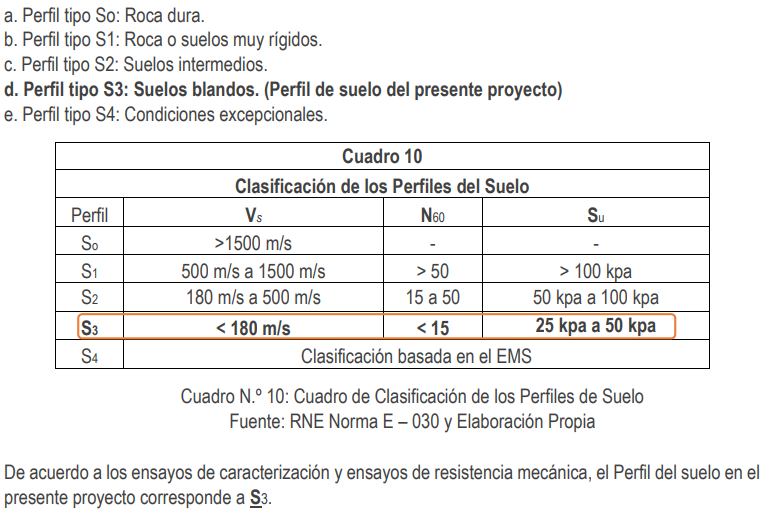
\includegraphics[scale=0.85]{IMAGENES/1.PNG}
    \caption*{\small Fuente: \it EMS}
    \label{fig:my_label}
\end{figure}

\newpage
\subsection{Profundidad de cimentación y capacidad portante}

\begin{figure}[h!]
    \centering
    \caption{Profundidad de cimentación}
    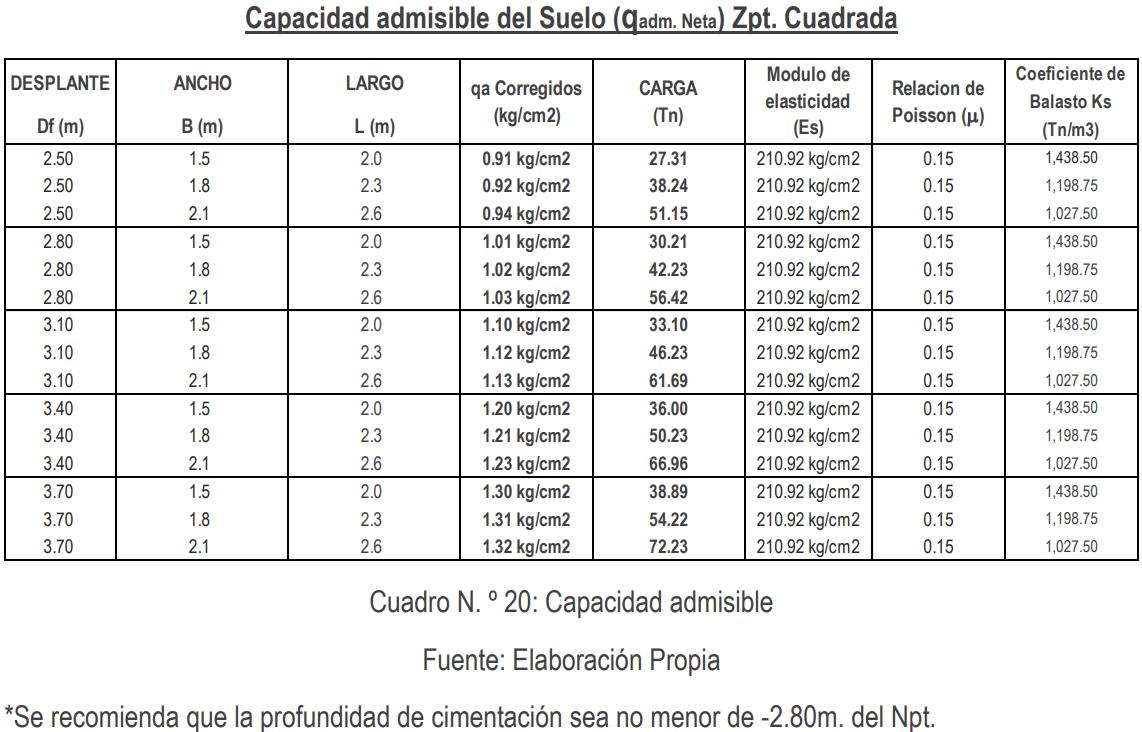
\includegraphics[scale=0.6]{IMAGENES/2.PNG}
    \caption*{\small Fuente: \it EMS}
    \label{fig:my_label}
\end{figure}

\section{Arquitectura}
Ver figuras \ref{pl} y \ref{el}.
\begin{figure}[h!]
    \centering
    \caption{Planta}
    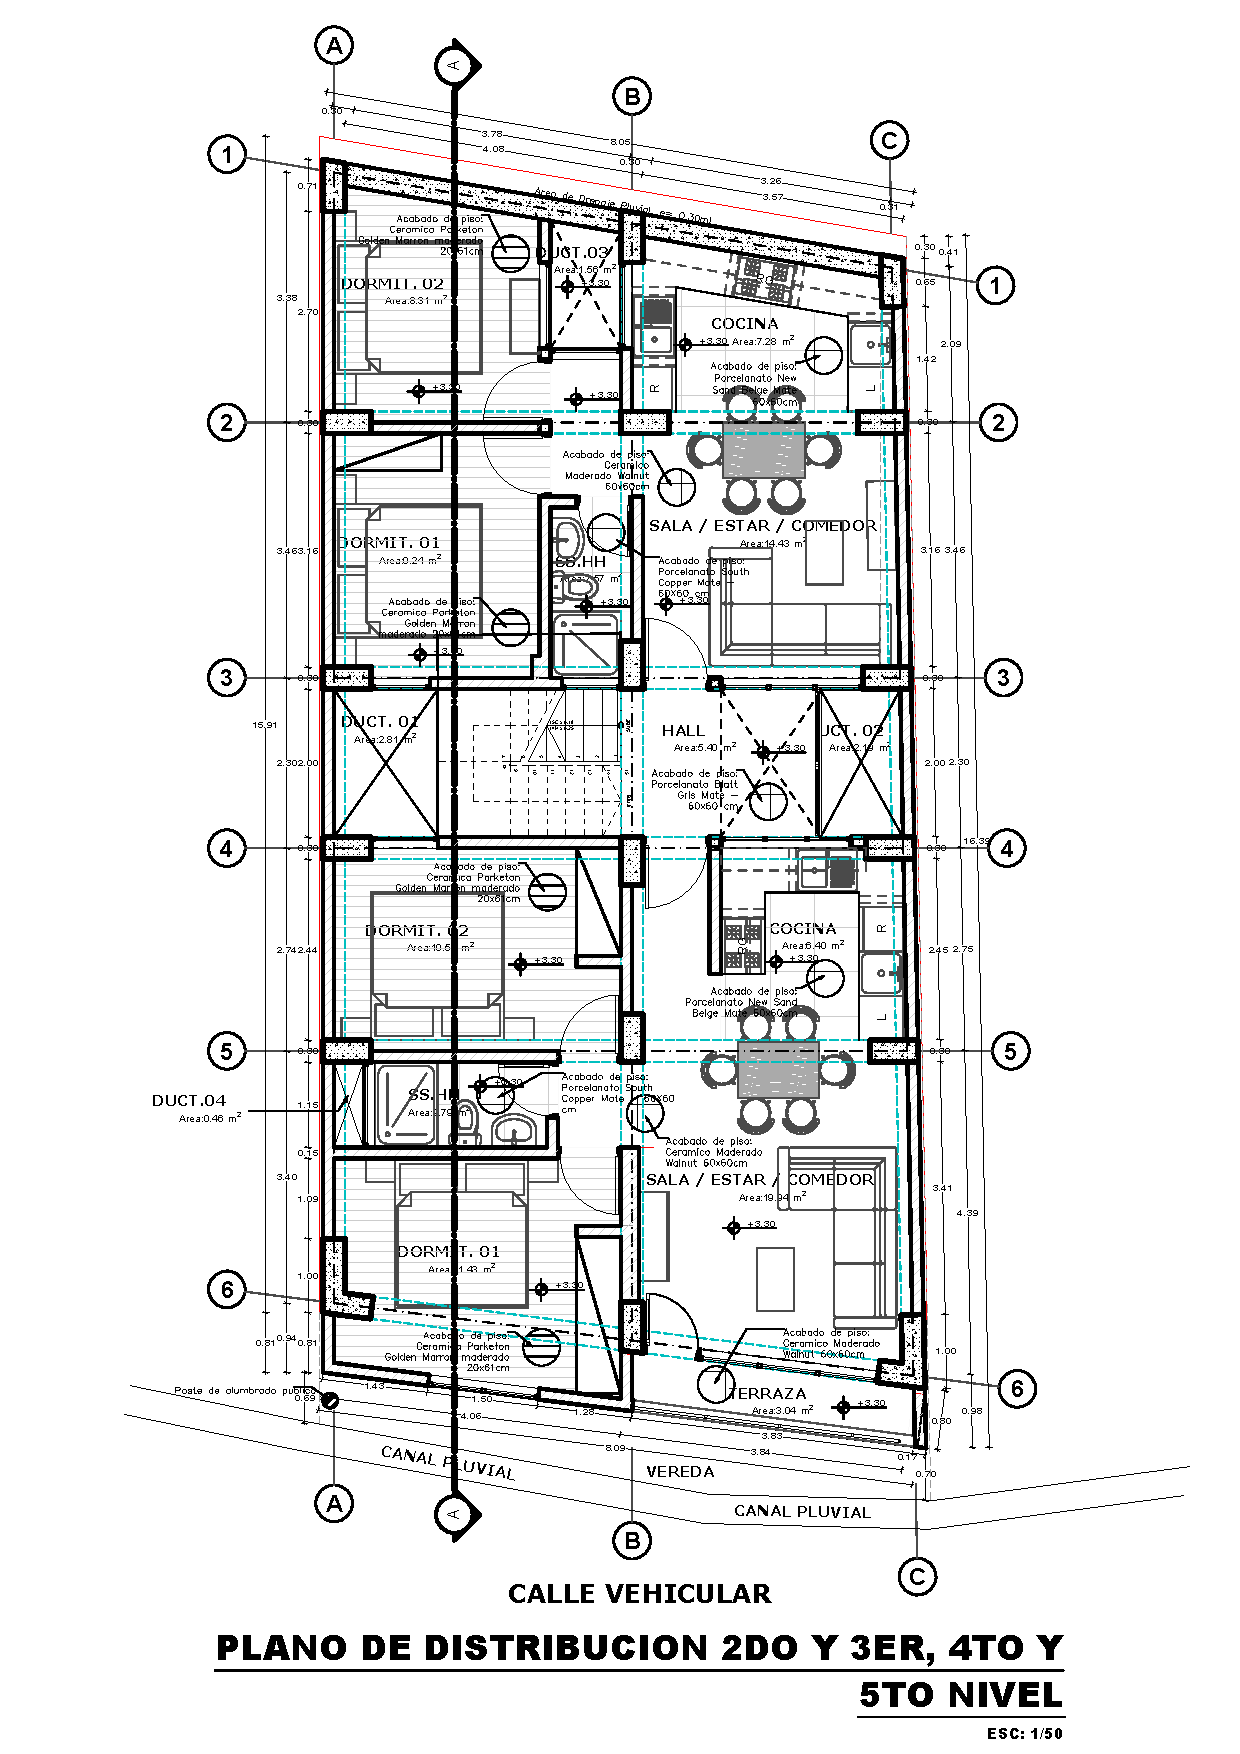
\includegraphics[scale=0.7]{IMAGENES/Plano.pdf}
    \label{pl}
\end{figure}

\begin{figure}[ht!]
    \centering
    \caption{Elevación}
    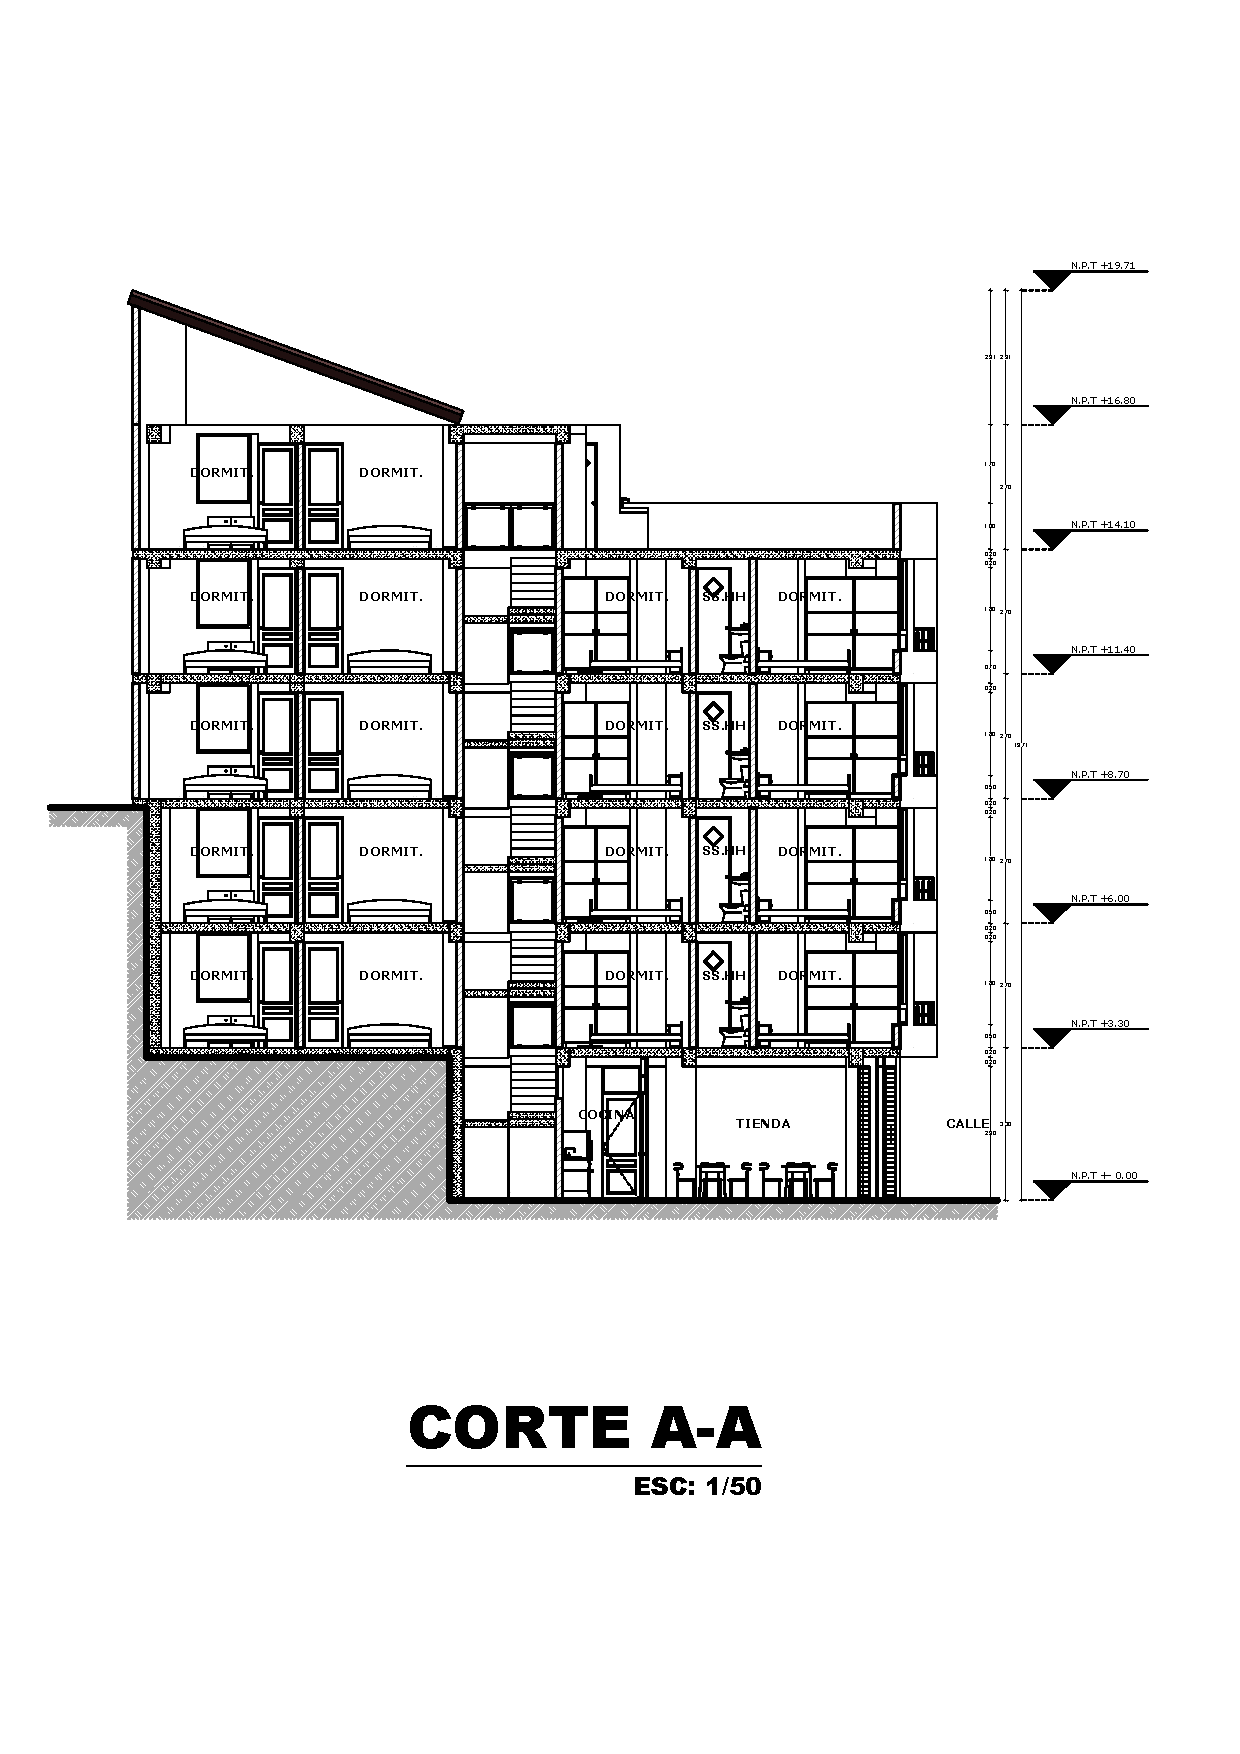
\includegraphics[trim={0 2cm 0 4.2cm},scale=0.7]{IMAGENES/ele.pdf}
    \label{el}
\end{figure}
%trim={<izquierda> <abajo> <derecha> <arriba>}
\section{Bases legales}
El desarrollo del presente trabajo se basa en las siguientes normas y reglamentos:
\begin{itemize}
  \item Norma Técnica de Edificación E.020 (Cargas)
  \item Norma Técnica de edificación E.030 (Diseño Sismoresistente)
  \item Norma Técnica de edificación E.050 (Suelos y Cimentaciones)
  \item Norma Técnica de edificación E.060 (Concreto Armado)
\end{itemize}

\var{b}